\documentclass[conference]{IEEEtran}

\usepackage[nolist]{acronym}
\usepackage[backend=bibtex]{biblatex}
\usepackage{graphicx}

\addbibresource{vision-transformer.bib}

\hyphenation{op-tical net-works semi-conduc-tor}


\begin{document}

\title{\acl{vit} Architectures with Registers (Thesis outline)}

\author{\IEEEauthorblockN{Florian Weidner}
	\IEEEauthorblockA{Philipps-University Marburg, Germany\\
		Department of Mathematics and Computer Science, Deep Learning Group\\
		February 09, 2024\\
}}

\maketitle
\begin{abstract}
The abstract goes here.
\end{abstract}

\begin{IEEEkeywords}
	\ac{vit}, 
	\end{IEEEkeywords}

\IEEEpeerreviewmaketitle

\section{Introduction}
Introduction to the topic...

Explanation of \acp{vit} \cite{10.1145/3505244} \cite{visiontransformers2021} \cite{ruan2022visiontransformersstateart} \cite{Liu2024-lm}

\section{Vision Transformers}

\begin{figure}
  \centering
  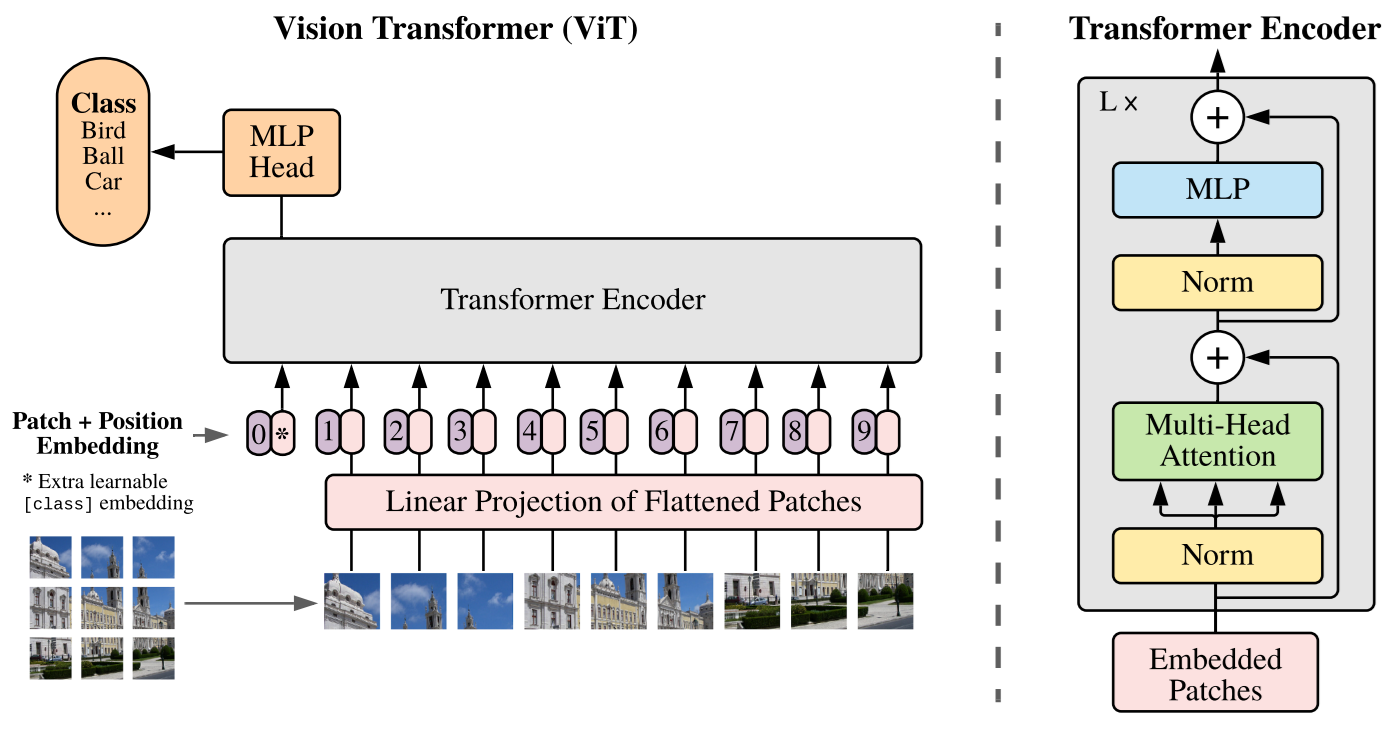
\includegraphics[width=0.5\textwidth]{figures/vit-architecture.png}
  \caption{Overview of a \ac{vit} architecture. \cite{visiontransformers2021}}
  \label{fig:vit-architecture}
\end{figure}

The Transformer architecture is a neural network model architecture, created primarily for sequence-to-sequence tasks in \ac{nlp}. It consists of an encoder, which makes the input sequence into a continuos representation and a decoder, which then generates the output sequence. The encoder is built up of n identical layers, containing following components:
\begin{itemize}
  \item multi-head self-attention mechanism: captures relationships between all tokens in the input, regardless of their distance
  \item feed-forward network: simple two-layer MLP network with ReLU activation which is applied to each token separately
  \item add \& norm layers using residual connections and layer normalization to stabilize the training
\end{itemize}
The result outcome of the encoder is a enriched sequence representation, which is then used by the decoder to generate the output sequence. The decoder also consits of n identical layers with:
\begin{itemize}
  \item masked multi-head self-attention mechanism: ensures a causal generation, by preventing that tokens have impact to future tokens
  \item encoder-decoder attention mechanism: focuses on the relevant parts of the encoder's output
  \item feed-forward network: similar to the encoder
  \item add \& norm layer:ssimilar to the encoder
\end{itemize}
The input text is embedded and combined with a positional encoding to provide token order information. Because several attention layers can run in parallel, the architecture is significantly more parappelizable than \ac{rnn} or \ac{cnn} architectures, which makes it very efficient for modern hardware accelerators. That allows the Transformer to scale to very large models and datasets. \cite{transformer2017}

\citeauthor{visiontransformers2021} introduced the idea of using the stated transformer architecture for computer vision. A lot of research tried to combine self-attention mechanisms with \ac{cnn} architectures, not achieving a effectively scalable method for modern hardware accelerators. \cite{visiontransformers2021} proposed to apply a standard Transformer directly to images, that are split into fixed-size patches. Each patch is flattened into a vector and passed through a linear projection layer to form an embedding as input for the Transformer. These embeddings are used as tokens in a \ac{nlp} scenario. Positional embeddings are added to retain spatial information since they process images as sequences, unlike \acp{cnn} which inherently capture spatial hierarchies. For classification tasks, an extra learnable [class] embeding is added in front of the embedded input. At the output of the encoder, the final representation of this token is used for classification. \acp{vit} have much less image-specific inductive bias than \acp{cnn}, because other than \acp{cnn}, with the global self-attention mechanism spatial relationships needs to learned from scratch, but long-range dependencies across the entire image can be captured. As Transformers, \acp{vit} are normally pre-trained on large datasets and then fine-tuned to more specific tasks. After pre-training, the prediction head is removed and a zero-initialized feedforeward layer,where the size is the number of classes, is added.
Like Transformers, \acp{vit} are also very parallelizable, which makes them very efficient. But \cite{visiontransformers2021} found out that without large-scale pre-training, \acp{vit} often underperform. So \acp{vit} requires sidnificant computational resources. But when pre-trained on large datasets, \acp{vit} outperforms \acp{cnn} on image classification tasks. The architecture performs well for transfer learning, where the pre-trained model can be fine-tuned already with limited labeled data. \cite{visiontransformers2021} \cite{visiontransformers2021} stated that further scaling of ViT would likely lead to improved performance.  Alo  self-supervised pre-training can be improved. They found out that with mimicking the masked language modeling task used in BERT, the model performs still better than \acp{cnn} but a bit worse that with supervised pre-training. By now different architectures and training-tricks of \acp{vit} have been proposed to further improve \acp{vit} including self-supervised learning.

The architecture got adapted for image recognition, object detection, image segmentation, pose estimation, and 3D reconstruction tasks. \cite{vit-state-challenges} 
\section{Vision Transformers need registers: A summary}
Summerization and explanation of the paper \cite{darcet2024visiontransformersneedregisters} \cite{wang2024mambarvisionmambaneeds}

\section{Comparison to other papers with performance improvements of \ac{vit}s}

\begin{figure}
  \centering
  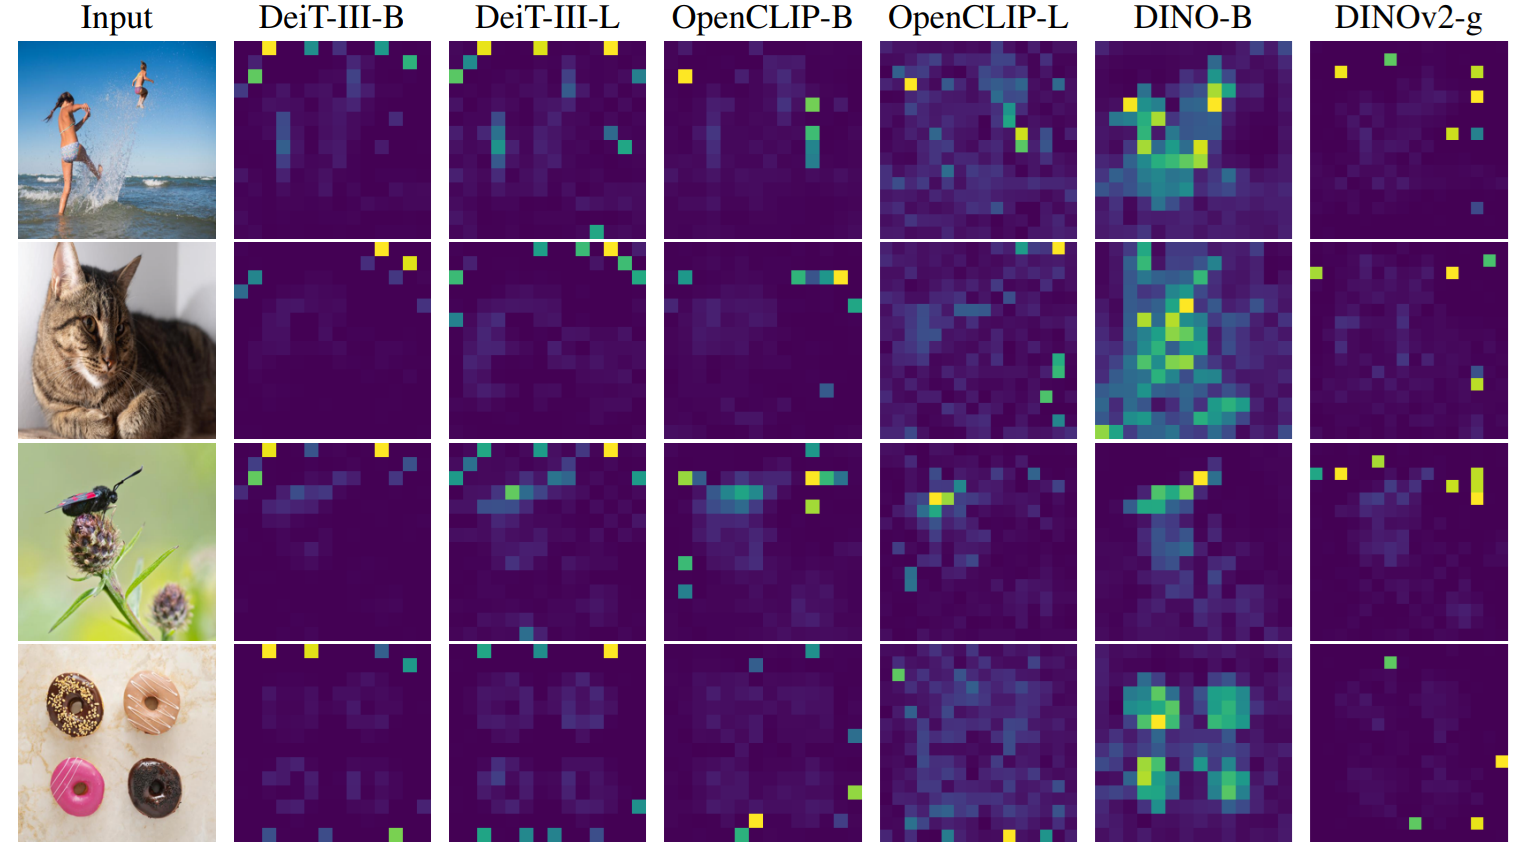
\includegraphics[width=0.5\textwidth]{figures/vits-artifacts.png}
  \caption{Illustration of artifacts observed in the attention maps of modern vision transformers. \cite{registers}}
  \label{fig:artifacts-observations}
\end{figure}

I this chapter we summerize the paper \cite{registers}. The paper discoverd artifacts and proposes to use additional register tokens for \acp{vit} to remove these artifacts.
After introducing to \acp{vit} like we did in this paper, the models they found the artifacts are introduced. The DINO algorithm is a self-supervised learning method, that uses two \acp{vit}. A student network is predicting the output of a teacher network, to learn rich representaions of visual data without the need of manual annotations. \cite{dino} DINO is shown to produce models, that contain semantically consistent information in the last attention layer. Object discovery algorihtms like LOST, built on top of DINO, are using these attention maps, that often contains semantically interpretable information, used to detect objects without supervision. DINOv2 \cite{dinov2} is a improved followup focusing on dense predition tasks, which are tasks, where detailed outputs are required to provide fine-grained localized informations, like semantic segementation or depth estimation. Despite good performance on these dense tasks, the authors observed that DINOv2 is incompatible with LOST \cite{registers}. The different behaviour of DINO and DINOv2 can be observed in the artifacts in the last attention maps. In figure \ref{fig:artifacts-observations} you can see the different models and their artifacts on the last attention layer.
While DINO shows no peak outlier values focusing the main object in the image, DINOv2 shows a lot of artifacts on the background of the images. This qualitatively observation can be also made for the label-supervised model DeiT-III and the text-supervised model OpenCLIP. Shown in figure \ref{fig:artifacts-observations}, you can observe similar artifacts in the background.
To explain why and where the artifacts of \acp{vit} in attention maps appear, the paper focuses on DINOv2. 
Artifact patches show higher norm of their token embedding at the output of the model than other patches. In figure \ref{fig:artifacts-norm} you can see the distribution of the local feature norms over a small dataset. While for DINO, the norm stays under 100 for all patches, DINOv2 shows a lot of patches with a norm higher than 150. This cutoff value can vary across different models. They define artifacts as
\begin{quote}
  "tokens with norm higher than 150 will be considered as “high-norm” tokens" \cite{registers}
\end{quote}

The authors found different conditions, when the artifacts appear in the training process of DINOv2. Figure \ref{fig:artifacts-layer} shows the following conditions:
\begin{itemize}
  \item artifacts start appearing around layer 15 to 40.
  \item artifacts start appearing after on thrid of training.
  \item artifacts only appear in the three largest model versions
\end{itemize}

Another discovery is that the high-norm tokens appear where patch information is redundant. The authors tested the cosine similarity between high-nomr tokens and their four neighbors, directly after the image is emebdded. They observed, that the high norm patches appear where their cosine similarity to the neighbors is high. Compared to the observations, that shows that artifacts appear mostly in the background of images, high-norm pathes seem to have redundant information, that the model can ignore, to achive similar scores at the output. 


\begin{figure}
  \centering
  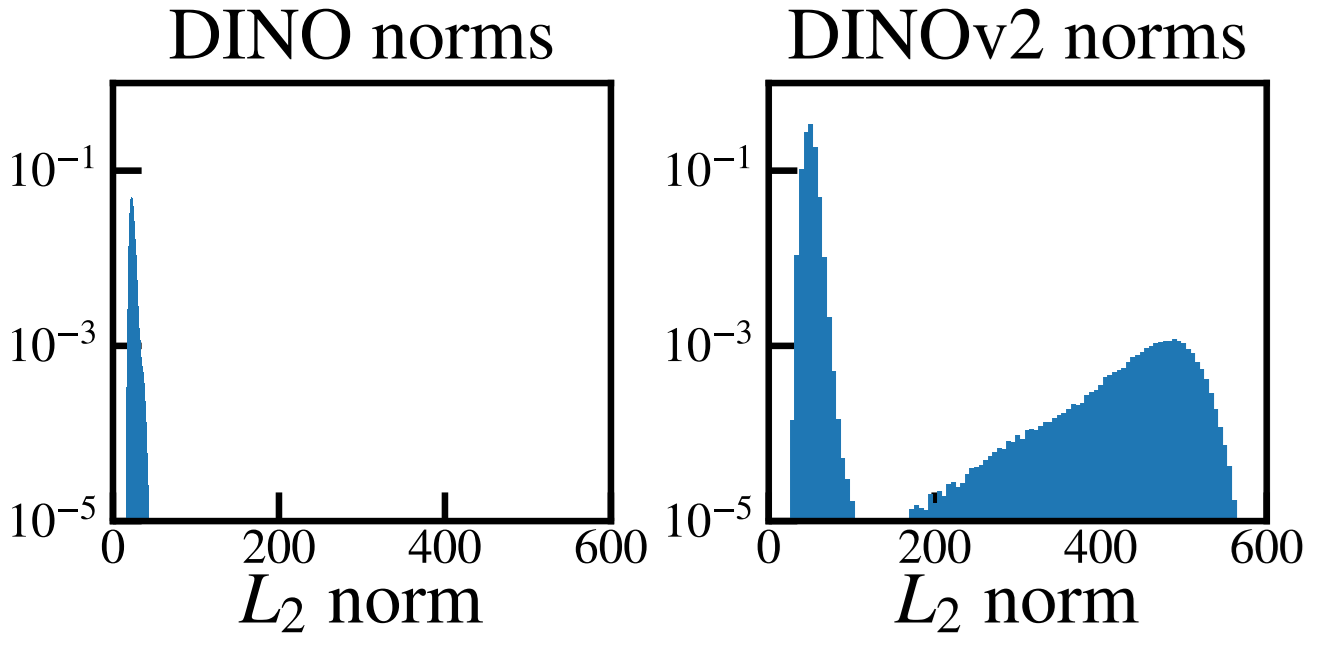
\includegraphics[width=0.3\textwidth]{figures/artifact-norm.png}
  \caption{Comparison of local feature norms for DINO ViT-B/16 and DINOv2 \cite{registers}}
  \label{fig:artifacts-norm}
\end{figure}

\begin{figure}
  \centering
  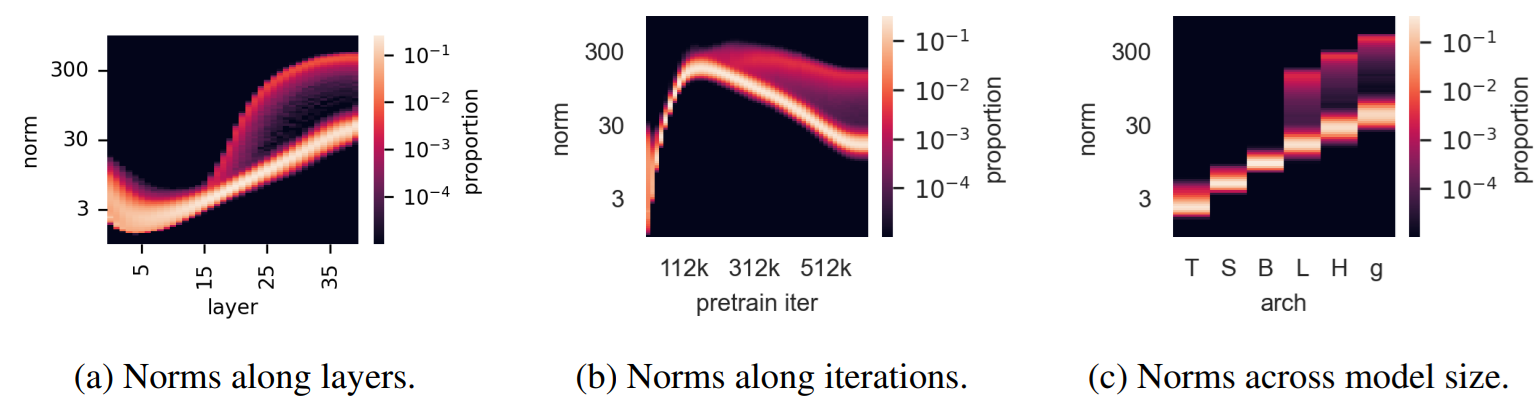
\includegraphics[width=0.5\textwidth]{figures/artifact-layers.png}
  \caption{Illustration of several properties of outlier tokens in the 40-layer DINOv2 ViT-g model \cite{registers}}
  \label{fig:artifacts-layer}
\end{figure}








survey: \cite{10.1145/3586074} 

I thought of comparing the previous explained paper \cite{darcet2024visiontransformersneedregisters} with papers like \cite{wen2024efficientvisionlanguagemodelssummarizing} \cite{Yin_2022_CVPR} \cite{10.1007/978-3-031-20053-3_30} \cite{ryoo2022tokenlearner8learnedtokens} \cite{Liu2024-lm} which try to improve efficiency of \ac{vit}s 

\section{Conclusion}
The conclusion goes here.

\printbibliography


\begin{acronym}
	\acro{vit}[ViT]{Vision Transformer}
  \acroplural{vit}[ViTs]{\ac{vit}s}
  \acro{nlp}[NLP]{Natural Language Processing}
  \acro{cnn}[CNN]{Convolutional Neural Network}
  \acroplural{cnn}[CNNs]{\acp{cnn}}
  \acro{rnn}[RNN]{Recurrent Neural Network}
  \acro{mlp}[MLP]{Multi-Layer Perceptron}
\end{acronym}


% that's all folks
\end{document}


